
% TODO bereinigen: "sao" vs "sau"
% TODO bereinigen: "tan-sao" vs "tan sao"


\newenvironment{WTSatz}[1]
	{\WTGaleryResetSlideshowCounter \subsection{#1}}
	{}

\newenvironment{WTSatzTeil}[2]
	{\paragraph{#1} (\textit{#2})}
	{}

\def\WTXFormen_EingangsGraphics#1{\includegraphics[width=2.5cm]{resources/images/eingangsform/#1}}


\def\WTSatzTechniken#1{\textbf{Ge\"ubte Techniken}: #1}

\def\WTKurzSatz#1#2#3{\paragraph{#1. #2} #3 (BILD!!! /resources/images/form/siunimtao/kurzsatz/#1.jpg)}

% XXXXXXXXXXXXXXXXXXXXXXXXXXXXXXXXXXXXXXXXXXXXXXXXXXXXXXXXXXXXXXXXXXXXXXXX



\renewcommand\chapterillustration{pushing_minimalistisch}
\chapter{Die Form}

Die Formen setzen sich aus einer Reihe von vordefinierten Bewegungsabl\"aufen zusammen, die von jedem WT-Praktizierenden regelm\"a{\ss}ig, aufmerksam und bewusst durchgef\"uhrt werden sollte. Die Art der Ausf\"uhrung hierbei kann gerne variieren: mal schnell/langsam, mal hart/weich, mal auf dem einen/anderen Bein, mit nur einer Hand, etc. Auf jeden Fall sollte nicht durch Hetzerei die Bewegung \textit{verwischt} werden, sondern jeder Punkt noch durchlaufen werden.

Nach l\"angerem \"Uben schleifen sich die Bewegungen ein und sind sofort f\"ur einen abrufbar. Dies gibt einem die M\"oglichkeit sich eine Art Werkzeugkasten zu bauen, aus dem man sich dann bei Bedarf bedient um eine konkrete Technik umzusetzen.

% TODO Ziel der Form ist es nicht wie bei einer japanischen Kata zum Beispiel gegen einen imagin\"aren Gegner zu k|\"ampfen

\newpage


\section{Begin und Schluss}
%%%%%%%%%%%%%%%%%%%%%%%%%%%%%%%%%%%%%%%%%%
%%%%%%%%%%%%%%%%%%%%%%%%%%%%%%%%%%%%%%%%%%


%\subsection{Eingangsform}

Die \textbf{Eingangsform} geht von einem lockeren Stand aus, und f\"uhrt in den sogenannten IRAS\index{IRAS}-Stand, was soviel bedeutet wie: \textit{\textbf{I}nternally \textbf{R}otated \textbf{A}dduction \textbf{S}tance}. Hierbei werden die Knie zueinandergepresst wobei die Oberschenkelmuskulator (die Adduktoren; v. lat.: \textit{adducere}, hinf\"uhren, hinziehen) durchgehend gespannt und somit trainiert werden. Dieser Stand versteht sich nur als Trainingsstand zur Verbesserung der Beinmuskulator und ist nicht gedacht zum Einsatz im Ernstfall.

\begin{figure}[htbp]
	\centering
	\begin{tabular}{ccccc}
		\WTXFormen_EingangsGraphics{arm1} & \WTXFormen_EingangsGraphics{arm2} & \WTXFormen_EingangsGraphics{arm3} & \WTXFormen_EingangsGraphics{arm3} & \WTXFormen_EingangsGraphics{arm3} \\
		\WTXFormen_EingangsGraphics{bein1} & \WTXFormen_EingangsGraphics{bein2} & \WTXFormen_EingangsGraphics{bein3} & \WTXFormen_EingangsGraphics{bein4} & \WTXFormen_EingangsGraphics{bein5} \\
		a) & b) & c) & d) & e) \\
	\end{tabular}
\end{figure}

Ausgangspunkt ist ein aufrecher, entspannter Stand a), der Blick ist nach vorne gerichtet, der Kopf sitzt weiter hinten, die Arme h\"angen locker auf der Seite hinunter, die F\"usse sind gschlossen und die H\"ande offen. Nun werden beide H\"ande zu F\"austen gemacht und dann der Seite entlang brusthoch angezogen b), die Fingerkn\"ocheln schauen nicht vor dem K\"orper und die Ellbogen nicht aus ihm heraus, die Unterarme sind parallel zum Boden. Dann werden die Knie gebeugt c) und man setzt sich leicht mit aufrechtem Oberk\"orper in die Hocke. Um den Stand zu verbreitern dreht man die Zehenspitzen so weit wie m\"oglich auf den Fersen auseinander d). Danach folgen die Fersen e) und werden \"uber die Fussmitte aufgemacht sodass beide F\"u{\ss}e ein gleichseitiges Dreieck am Boden formen.
	
	
	\begin{WTCommonBegriff}
		Oder auch auf Chinesisch \textit{Yee-Gee-Kim-Yeung-Ma} mit w\"ortlicher \"Ubersetzung Schriftzeichen-Zwei-Adduktions-Stand.
		% TODO erklaerung warum symbol 2, mit grafik
	\end{WTCommonBegriff}
	
\begin{WTCommonNoob}
	Man dreht gerne auf den Zehen auseinander was zu einem falschen Stand f\"uhrt.
\end{WTCommonNoob}

\WTGaleryImageTwo{eingangsform/fertig-front}{eingangsform/fertig-seite}{Demonstration des IRAS Stand}

%\subsection{Ausgangsform}

Am Ende gibt es dann eine kurzgehaltene \textbf{Ausgangsform} die wieder zur\"uck in einen lockeren Stand f\"uhrt:

\begin{WTalphenum}
	\item Ausgangspunkt ist der volle IRAS Stand.
	\item Als erstes wird der rechte Fuss gerade gestellt, sodass Zehen und Ferse eine gerade Linie nach vorne bilden.
	\item Nun stellt (noch immer gehockt) der linke Fuss zum rechten parallel Fuss mit kleinem Abstand zu.
	\item Erst jetzt werden die Beine aus der Hocke gestreckt.
	\item Und zu letzt werden die Arme an der Seite locker hinuntergef\"uhrt.
\end{WTalphenum}


\section{Siu-Nim-Tau}
%%%%%%%%%%%%%%%%%%%%%%%%%%%%%%%%%%%%%%%%%%
%%%%%%%%%%%%%%%%%%%%%%%%%%%%%%%%%%%%%%%%%%
% http://everything2.com/title/Sil+Lum+Tao

Siu-Nim-Tau bedeutet so etwas wie \textit{Kleine Idee} oder auch \textit{kleine Ideen Form}. Klein deshalb, da man recht isolierte Bewegungen ausf\"uhrt und sich auf das kleine, die Details konzentriert. So gibt es in dieser Form z.B. keinerlei Wendungen oder Schritte, der Oberk\"orper und die Beine bleiben durchgehend in der selben Position und bewegen sich nicht, sondern nur die Arme und H\"ande f\"uhren die Aktionen aus.

Ziel ist es hier f\"ur den Anf\"anger lernen sich zu entspannen, seine Schultern unten zu lassen und locker sein. Weiters wird einem gelehrt wo sich seine (K\"orper-) Mitte befindet. So wird z.B. das zur Mitte stellen der Faust im 2. Satz sehr betont, oder das Zur\"uckziehen eines seitlichen Pak Saos zur Zentrallinie. Wobei hier auch das K\"orperende gleichzeitig aufgezeigt wird. So sollen die Techniken nicht weiter nach au{\ss}en als die Schulter, oder h\"oher als das Ohr (6. Satz Lau Sao) bzw tiefer als der Genitalbereich (4. Satz Gum Sao) gehen. Es bildet sich damit ein Rechteck dass den K\"orper von Au{\ss}en und Innen trennt und in dessen Mitte sich die Zentrallinie befindet.

% TODO wie schreibt man dim-dim-chin ?
Das Motto der SNT ist \textit{Punkt-Punkt-Klar}. Es sollen jede Stationen (Punkte) der Bewegungen klar ersichtlich erreicht werden. Ein Nehmen von Abk\"urzungen ist also nicht angebracht und verf\"alschen den Ablauf. Weitere Mottos\footnote{aus dem Buch XXX TODO XXX} die beim \"Uben helfen:

\begin{itemize}
	\item Dr\"ucke deinen Kopf Richtung Himmel und stehe fest am Boden.
	\item Kopf hoch mit horizontalem Blick.
	\item Aufnahmef\"ahiger Brustkorb und aufgerichteter R\"ucken.
	\item H\"ufte gerade und Bauch einziehen
	\item Bei allen Bewegungen der Arme zu beachten: Tiefer Ellbogen und entspannte Schulterhaltung
	\item Wenn eine Armbewegung erfolgt: Schau in die Richtung der Handbewegung.
\end{itemize}

\begin{WTCommonBegriff}
	Siu-Nim-Tau kann auch geschrieben werden als \textit{Siu-Lin-Tau} (ein bisschen am Anfang \"uben) oder als \textit{Siu-Lam-Tau} (Vergiss nicht, dass der Ursprung des wing chun im Shaolin liegt)
\end{WTCommonBegriff}

\subsection*{Die acht S\"atze im \"Uberblick\footnote{\textit{Achtung}: Die Betitelung der einzelne S\"atze ist eine pers\"onliche Merkhilfe und Versch\"onerung welche gerne in anderen Kampfk\"unsten auch vorgenommen werden, die aber so im Unterricht der EWTO nicht anzufinden ist. Vielmehr werden die S\"atze einfach anhand ihrer Nummer 1-8 benannt.}}

\WTKurzSatz{1}{Schneidende Arme}{Vorne \"uberkreuzen und runterschneiden}
\WTKurzSatz{2}{Einfacher Fauststo{\ss}}{B}
\WTKurzSatz{3}{Dreifache Verehrung}{B}
\WTKurzSatz{4}{Lange Br\"ucke}{B}
\WTKurzSatz{5}{Mit der offenen Hand schlagen}{B}
\WTKurzSatz{6}{Ein D malen}{B}
\WTKurzSatz{7}{Schwingen ausbreiten}{B}
\WTKurzSatz{8}{Befreiungssatz}{B}

\textbf{Achtung: } In den folgenden Abbildungen sind s\"amtliche seitengleiche S\"atze nur einmal f\"ur links dargestellt, da sich die andere Seite recht schnell selbst herausfinden lassen sollte. Nicht betroffen sind nat\"urlich davon die S\"atze bei denen beide Arme zum Einsatz kommen (1., 4. und 8.), wobei man diese nat\"urlich auch gerne von Zeit zu Zeit seitenverkehrt ausf\"uhren kann.


\begin{WTSatz}{Schneidende Arme}% 1. SATZ
%%%%%%%%%%%%%%%%%%%%%%%%%%%%%%%%%%%%%%%%%%

	\WTSatzTechniken{Tan-Sao, Gan-Sao}

	\begin{WTSatzTeil}{Gau-Cha-Tan-Sao}{Gekreuzte Handfl\"achen nach oben H\"ande}
		\WTGalerySlideshowFour{siunimtau/1/1}{siunimtau/1/2}{siunimtau/1/3}{siunimtau/1/3b}
		
		Als allererstes werden beide geschlossene F\"auste a) ganz ge\"offnet sodass die Handfl\"achen eine gerade Oberfl\"ache bilden b). Danach werden die H\"ande, gef\"uhrt von den Ellbogen (welche zu der Zeit bereits eine gewisse Vorspannung besitzen) nach vorne geschoben c) bis dass ein Abstand von einer Faust breit zwischen K\"orper und Ellbogen besteht, und die Fingerspitzen auf H\"ohe der Schultern sind d). Um korrekte Winkeln zu gew\"ahrleisten sollte noch gepr\"uft werden, ob die Hautlinien beim rechten Handgelenk gerade noch sichtbar sind, und die Ellbogen seitlich mit dem K\"orper abschliessen.
		
		Der sogenannte \textit{gekreuzte Tan-Sao} ist in beidh\"andiger Ausf\"uhrung nur in der Form zu sehen, da er wenn dann nur einarmig und in gewendeter Position Anwendung findet. Man kann dies ganz einfach nachpr\"ufen in dem man eine Hand wegnimmt, und eine Wendung durchf\"uhrt.
		
		%TODO bild von einarmig-gekreuzten tan sao in wendung
		%TODO bild von hautlinie die gerade mit hand abschliesst fuern gekreuzten-tan sao
	\end{WTSatzTeil}
	
	\begin{WTSatzTeil}{Gau-Cha-Gan-Sao}{Gekreuzte schneidende Arme}
		\WTGalerySlideshowTwo{siunimtau/1/3}{siunimtau/1/4}
		
		Startend im doppelten Tan-Sao e) schneidet der Gan-Sao (nicht zu verwechseln mit dem Gam-Sao) mit der Elle eine gerade Linie hinunter f), so als w\"urden die Arme etwas abschneiden wollen, und beschreibt \textbf{nicht} in einer Wischbewegung einen Kreis! Darum wird auch geraten die Bewegung nicht bewusst zu steuern, sondern einfach nur die Arme locker fallen lassen. Am Ende wird der Unterarm leicht nach au{\ss}en routiert so dass man auch wirklich mit dem Knochen auftrifft.
	\end{WTSatzTeil}
	
	\begin{WTSatzTeil}{Kwan-Sao}{Rotierender Arm}
		\WTGalerySlideshowThree{siunimtau/1/4}{siunimtau/1/5}{siunimtau/1/6}
		
		Ausgehend vom fertigen Gan-Sao g) werden die Arme nach oben rotiert h), wobei die H\"ande nahe am K\"orper entlang angehoben werden. Der linke Arm dreht sich dabei unter dem Rechten durch und befindet sich dann weiter innen.
		
		Am Schluss der Bewegung befindet man sich exakt wieder in der urspr\"unglichen Tan-Sao Position i) mit der linken Hand oben.
		
		\begin{WTCommonNoob}
			Beim Kwan-Sao werden Handgelenke nicht abgewinkelt, sondern bleiben eine geradlinige Verl\"angerung des Unterarms. Um Platz zu machen f\"uhr die L\"ange der Arme muss man die \textbf{Ellb\"ogen} leicht \textbf{nach aussen} schieben.
		\end{WTCommonNoob}
	\end{WTSatzTeil}
	
	\begin{WTSatzTeil}{Sau-Kuen}{Ellbogen nach Hinten}
		\WTGalerySlideshowThree{siunimtau/1/6}{siunimtau/1/7}{siunimtau/1/8}
		
		Ausgehend vom Tan-Sao j) wird mit beiden H\"anden gleichzeitig eine Faust gemacht k) und dann stossen die Ellb\"ogen dynamisch nach hinten, sodass die F\"auste wieder auf Brusth\"ohe sind l).
	\end{WTSatzTeil}
	
\end{WTSatz}

%%%%%%%%%%%%%%%%%%%%%%%%%%%%%%%%%%%%%%%%%%

\begin{WTSatz}{Einfacher Fauststo{\ss}}% 2. SATZ
	
	\WTSatzTechniken{Chung-Kuen}
	
	\begin{WTSatzTeil}{Yat-Gee-Chung-Kuen}{Fauststoss}
		\WTGalerySlideshowFour{siunimtau/2/1}{siunimtau/2/2}{siunimtau/2/3}{siunimtau/2/4}
		
		Am Anfang des zweiten Satzes a) wird, noch bevor etwas anderes passiert, die linke Faust an ihrem Platz in die Vertikale gedreht b). Nun besetzt die Faust nahe am K\"orper die Zentrallinie c) wobei die Auftreffsfl\"ache schon gerade nach vorne zeigt. Zu guter Letzt wird der Arm gestreckt d) in dem der Ellbogen die Bewegung anf\"uhrt. Der Schlag soll nicht verkrampft ausgef\"uhrt werden, als auch kein Bizeps kommt zum Einsatz. Stattdessen spannt der K\"orper nur ganz am Anfang der Bewegung und ganz kurz vor dem Aufschlag; w\"ahrend der \textit{Flugzeit} ist der Arm locker. Auch die Kraft kommt mehr vom Trizeps und dem R\"ucken, wobei auch gerne der Lat bewusst \"uberm\"a{\ss}ig angespannt sein kann um ein Mitgehen der Schulter zu verhindern.
		
		Diese \"Ubung soll einem zeigen wo sich eigentlich seine Mitte befindet. Die Siu Nim Tau zeigt einem damit die Grundlagen und Positionen von seinem K\"orper. Man lernt quasi sich selbst einmal kennen, um dann sp\"ater auch andere kennen zu lernen $;)$
		
	\begin{WTCommonBegriff}
		Die im WT verwendete vertikale Faust wird im Chinesischen auch als \textit{Sonnenzeichen-Faust} bezeichnet, da das Symbol f\"ur Sonne den Konturen der Faust sehr \"ahnlich sieht:
		
		\center{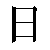
\includegraphics[width=1cm]{resources/graphics/chinese_sun_symbol}}
		\flushleft
		
		Die Aneinanderreihung von mehreren Sonnenzeichen-F\"austen ist eine Spezialit\"t im WT und wird als \textit{Ketten-Faustst\"osse} bezeichnet.
	\end{WTCommonBegriff}
			
		% TODO referenz hinzu: Siehe Anatomie des Fauststoss.
		
		% TODO pruefung stoss von vorne auf faust, a la gernot
		
	\end{WTSatzTeil}
	\begin{WTSatzTeil}{Tan-Sao, Huen-Sao, Sao-Kuen}{Handfl\"ache-oben Hand, Zirkelnde Hand, Ellbogenstoss}
	
		Diese \textbf{Schlusssequenz}\index{Schlusssequenz} findet sich am Ende von (fast) jedem Satz und besteht aus folgende f\"unf Bewegungen:
		
		
		\WTGalerySlideshowThree{siunimtau/2/5}{siunimtau/2/6}{siunimtau/2/7}
		
		
		Ausgangspunkt ist ein Tan-Sao e) von dem aus die Finger einklappen und die Spitzen den Unterarm greifen wollen f). Danach folgt eine halbe Umdrehung der Hand (Huen-Sao) g) bis mindestens ganz nach unten; eine Drehung weiter nach aussen w\"urde zu einer zus\"atzlichen Dehnung f\"uhren und simuliert somit eventuell besser das folgende Greifen im n\"achsten Schritt h).
		
		\WTGalerySlideshowThree{siunimtau/2/8}{siunimtau/2/9}{siunimtau/2/10}
		
		Ob nun zuerst die Faust gedreht wird i) oder zeitgleich mit dem Zur\"uckziehen ist mehr eine pers\"onliche Preferenz und kann von Lehrer zu Lehrer unterschiedlich sein.
		
		Wichtig ist hierbei den Arm durchgehend bei jeder Bewegung \textbf{durchgestreckt} zu lassen und nicht abzuwinkeln.
		
	\end{WTSatzTeil}
\end{WTSatz}

%%%%%%%%%%%%%%%%%%%%%%%%%%%%%%%%%%%%%%%%%%

\begin{WTSatz}{Dreifache Verehrung}% 3. SATZ
	
	\WTSatzTechniken{Tan-Sao, Huen-Sao, Wu-Sao, Fook-Sao, Pak-Sao}
	
	Der dritte Satz ist (gemeinsam mit dem vierten) der l\"angste Satz der Form. Noch dazu kommt, dass die Ausf\"uhrung vergleichsweise langsam von statten geht und die Armbewegung synchron mit der Atmung sein soll.
	
	\begin{WTSatzTeil}{Tan-Sao}{Handfl\"ache-oben Hand}
		\WTGalerySlideshowFour{siunimtau/3/1}{siunimtau/3/2}{siunimtau/3/3}{siunimtau/3/4}
		
		Von der Grundstellung aus a) wird die linke Handfl\"ache ge\"offnet b) und nahe am K\"orper entlang zur Mitte bewegt. Von dort schl\"angelt sich die Hand weiter geradlinig nach vorne c), so als ob ein Hindernis \"ueberwunden werden m\"usste, bis die Tan Sao Endposition erreicht ist d). Die offene Handfl\"ache des Tan-Sao ist hierbei komplett gerade und parallel zum Boden, der Daumen anliegend.
% TODO grafik reingeben, wo stange ist und handbewegung eingezeichnet wie drumherum bewegt wird
		
	\end{WTSatzTeil}
	\begin{WTSatzTeil}{Huen-Sao}{Zirkelnde Hand}
		\WTGalerySlideshowFour{siunimtau/3/5}{siunimtau/3/6}{siunimtau/3/7}{siunimtau/3/8}
		
		Nun werden die Fingerspitzen nach Oben zu sich gezogen e) und von der Position aus ein Halbkreis nach rechts beschrieben f). Unten angekommen stellt die Hand sich nach vorne hin \textit{Finger f\"ur Finger} auf, bis eine Sperre im Handgelenk ein Weiterdrehen unm\"oglich macht g). Erst dann wird der Ellbogen etwas nach au{\ss}en gedreht sodass die Handfl\"ache kerzengerade nach Oben zeigt h). Es gilt hierbei zu beachten dass man im Spiegel nur den kleinen Finger sieht und sich alle anderen Finger quasi dahinter verstecken. Auch kann man die letzte Drehbewegung etwas mit der Handkante betonen um diesen speziellen Angriff zu trainieren.
		
		\begin{WTCommonBegriff}
			Da es sich hier um eine halbkreis, und keine ganzkreis Drehung handelt, wird diese Bewegung eigentlich genauer als \textit{Bon Huen Sao}\index{Huen Sao!Bon Huen Sao} bezeichnet.
		\end{WTCommonBegriff}

	\end{WTSatzTeil}
	\begin{WTSatzTeil}{Wu-Sao}{Sch\"utzende Hand}
		\WTGalerySlideshowTwo{siunimtau/3/8}{siunimtau/3/9}
		
		Mit aufgestellter Hand i) zieht man nun den Arm nach Hinten, so dass die Hand ungef\"ahr eine Faust vom K\"orper entfernt stehen bleibt j). Die Konzentration ist dabei beim geradlinig nach hinten ziehenden Ellbogen, von dem aus die Bewegung angesteuert wird.
		
	\end{WTSatzTeil}
	\begin{WTSatzTeil}{Fook-Sao, Huen-Sao, Wu-Sao x3}{Br\"uckenarm, Zirkelnde und Sch\"utzende Hand}
		\WTGalerySlideshowFour{siunimtau/3/9}{siunimtau/3/10}{siunimtau/3/11}{siunimtau/3/6}
		
		Der folgende Abschnitt stellt die eigentliche Verehrung dar und wird gezeigt in dem man \textbf{dreimal} die Bewegungen f) bis n) \textbf{wiederholt}. Gez\"ahlt hierbei werden die Anzahl der Fao-Sao Techniken, und nicht etwa der Wu-Sao, womit man auf vier mal kommen w\"urde.

% TODO die grafiken f-n) irgendwie hervorheben, weil sie sich 3x wiederholen; mit extra border ode rso
		
		Beginnend mit der Wu-Sao k) l\"asst man das Handgelenk vollkommen locker nach unten fallen l), so als ob man den Motor abrupt absterben hat lassen. Es soll aber das \textbf{Handgelenk nicht nach oben} bewegt werden. Dies trainiert die F\"ahigkeit den K\"orper isoliert steuern zu k\"onnen, wo ein Teil sich bewegt, der andere jedoch ruhig bleibt.

		Als n\"achstes schiebt die Hand nach vorne in den Fook Sao m). Der Ellbogen wandert hierbei so weit als m\"oglich in die K\"orpermitte, m\"oglichst soll weiter Innen als das Handgelenk. W\"ahrend der Bewegung versucht man mit der Hand seinen Unterarm zu greifen um so die dortige Muskulator zu trainieren und zieht mit den Fingern gerade nach vorne so als ob man eine Schnur aus seinem Unterleib ziehen w\"urde. Beachtenswert ist auch die Tatsache dass hier drei Kr\"afte gleichzeitig wirken: Das nach unten Ziehen der Schulter, das nach Innen Ziehen des Ellbogens, und das nach vorne Ziehen des gesamten Armes was zu einer gewissen Spannung f\"uhren kann.

% TODO foto von der hand von oben wenn man im fook sao ist; ist quasi eine schnabel hand (daumen liegt auf zeigefinger, bzw bissi auch mittelfinger); oben glatt als koennte man ein wasserglas draufstellen

		Durch das Drehen der Hand nach unten mit dem Huen Sao n) befindet man sich wieder exakt in der selben Position wie in f) und die gesamte Sequenz wird noch zwei mal wiederholt.
		
		\begin{WTCommonBegriff}
			Der sich wiederholende Teil wird auch \textit{dreifache Verehrung Buddhas}\index{Dreifache Verehrung Buddhas} genannt, was im Originalen mit \textit{Sam Bai Fat}\index{Sam Bai Fat} (oder auch \textit{Fat Shan} in Kantonesisch) \"ubersetzt wird. Der \"Ubende soll hier also einen gro{\ss}teil seiner Aufmerksamkeit nach Innen richten was der Bewegung einen eher meditativen Aspekt verleiht.
		\end{WTCommonBegriff}
	
	\end{WTSatzTeil}
	\begin{WTSatzTeil}{Seitlicher Pak Sao}{Handfl\"achenstoss}
		\WTGalerySlideshowTwo{siunimtau/3/9}{siunimtau/3/20}
		
		Ausgehend von der Wu Sao o) wird die Handfl\"ache bis zur Schulter (welche zugleich das K\"orperende darstellt) bewegt, dabei bleibt der gesamte Arm n\"aher am K\"orper und bewegt sich auf einer parallelen Linie. Um dem WT Prinzip folge zu leisten, welches besagt dass der Blick der Technik folgen soll, bewegen sich die Augen in die sto{\ss}ende Richtung.
		
		\begin{WTCommonBegriff}
			 Der seitliche Pak Sao im dritten Satz wird in der Fachliteratur auch gerne als \textit{Djark Cheung}\index{Cheung!Djark Cheung} bezeichnet, also \textit{seitlicher Handfl\"achenstoss}.
		\end{WTCommonBegriff}
		
	\end{WTSatzTeil}
	\begin{WTSatzTeil}{Ching Cheung\index{Cheung!Ching Cheung}}{Gerader Handfl\"achenstoss}
		\WTGalerySlideshowThree{siunimtau/3/21}{siunimtau/3/22}{siunimtau/3/23}
		
		Die erste Bewegung bereitet den n\"achsten Handfl\"achenstoss vor indem die Hand zur Mitte gezogen wird q). Dabei zeigt schon die Handfl\"ache in Richtung Gegner nach vorne, \"ahnlich wie beim zweiten Satz beim Hereinziehen der Faust zur Mitte. Zum Schluss wird einfach der Arm durchgestreckt r) und die Handkante entlang dem kleinen Finger betont. Ab dann dreht man in den Tan Sao s) und es wird wieder die typische \textbf{Schlusssequenz} ausgef\"uhrt.
		
	\end{WTSatzTeil}
	
\end{WTSatz}

%%%%%%%%%%%%%%%%%%%%%%%%%%%%%%%%%%%%%%%%%%

\begin{WTSatz}{Lange Br\"ucke}% 4. SATZ

	\WTSatzTechniken{Gum-Sao, Lan-Sao, Fak-Sao, Djut-Sao, Tok-Sao, Biu-Tze-Sao}
	
	\begin{WTSatzTeil}{Jor-/Yau-Gam-Sao}{Linke und rechte Hinunterdr\"uckende Arme}
		\WTGalerySlideshowThree{siunimtau/4/1}{siunimtau/4/2}{siunimtau/4/3}
		\WTGalerySlideshowTwo{siunimtau/4/4}{siunimtau/4/5}
		
		Asdf
	\end{WTSatzTeil}
	\begin{WTSatzTeil}{Hau-/Chin-Gam-Sao}{Hinten und Vorne Dr\"uckende Arme}
		\WTGalerySlideshowThree{siunimtau/4/6}{siunimtau/4/7}{siunimtau/4/8}
		\WTGalerySlideshowTwo{siunimtau/4/9}{siunimtau/4/10}
		Asdf
	\end{WTSatzTeil}
%		\WTGalerySlideshowFour{siunimtau/4/11}{siunimtau/4/12}{siunimtau/4/13}{siunimtau/4/14}
	\begin{WTSatzTeil}{Shang-Lan-Sao, Shang-Fak-Sao}{Doppelter Riegelarm, Doppelter Handkantenschlag}
		\WTGalerySlideshowThree{siunimtau/4/14}{siunimtau/4/15}{siunimtau/4/16}
		
		Zuerst Lan, dann schauen, dann Fak, dann zurueck Lan mit rechts oben.
		
		ellbogen fuehrt.
	\end{WTSatzTeil}
	\begin{WTSatzTeil}{Shang-Djam-Sao}{Doppelt sinkende Ellb\"ogen}
		\WTGalerySlideshowTwo{siunimtau/4/17}{siunimtau/4/18}
		
		asdf.
	\end{WTSatzTeil}
	\begin{WTSatzTeil}{Shang-Tan/Tok-Sao}{Doppelt XXX}
		\WTGalerySlideshowTwo{siunimtau/4/19}{siunimtau/4/20}
		
		asdf.
	\end{WTSatzTeil}
	\begin{WTSatzTeil}{Shang-Djat-Sao, Shang-Biu-Tze-Sao}{Doppelt ???, Doppelte Fingerstiche}
		\WTGalerySlideshowThree{siunimtau/4/21}{siunimtau/4/22}{siunimtau/4/23}
		
		asdf.
	\end{WTSatzTeil}
	\begin{WTSatzTeil}{Cheung-Kiu-Gam-Sao}{Lange Br\"ucke Gam-Sao}
		\WTGalerySlideshowTwo{siunimtau/4/23}{siunimtau/4/24}
		
		asdf
	\end{WTSatzTeil}
	\begin{WTSatzTeil}{Shang-Tai-Sao}{Doppelter ???}
		\WTGalerySlideshowFour{siunimtau/4/25}{siunimtau/4/26}{siunimtau/4/27}{siunimtau/4/28}
		
		asdf
	\end{WTSatzTeil}
	\begin{WTSatzTeil}{Huen-Sao, Sao-Kuen}{Schlusssequenz}
		
		mit verkehrtem, doppelten huen-sao.
	\end{WTSatzTeil}
\end{WTSatz}

%%%%%%%%%%%%%%%%%%%%%%%%%%%%%%%%%%%%%%%%%%

\begin{WTSatz}{Mit der offenen Hand schlagen}% 5. SATZ

	\WTSatzTechniken{Pak-Sao, Handfl\"achenstoss}
	
	\begin{WTSatzTeil}{Seitlicher Pak Sao}{Handfl\"achenstoss}
		\WTGalerySlideshowThree{siunimtau/5/1}{siunimtau/5/2}{siunimtau/5/3}

		Diese Bewegung (auch \textit{Djark Cheung} statt Pak Sao genannt) ist sehr \"ahnlich dem Schluss vom dritten Satz, wobei in diesem Fall der Winkel im Ellbogen ein etwas gr\"o{\ss}er ist. Von der Ausgangsstellung aus a) \"offnet sich die Hand b) und stosst sogleich zur Seite bis zur Schulter (K\"orperende).
		
		% TODO bild von oben, welcher winkel im gegensatz zu satz 3 zeigt
		
	\end{WTSatzTeil}
	\begin{WTSatzTeil}{Wang-Cheung}{Liegender/Horizonatler Handfl\"achenstoss}
		\WTGalerySlideshowThree{siunimtau/5/4}{siunimtau/5/5}{siunimtau/5/6}
		
		Die Hand wird bis zur Zentrallinie zur\"uck gef\"uhrt d) wobei die Handfl\"ache, vorbereitend f\"ur den n\"achsten Schlag, schon zur Seite gekippt wird. Dann wird einfach der Arm ausgestreckt und mit einer liegenden offenen Hand geschlagen e). Zur\"uck zum Tan Sao und man befindet sich wieder in der \textbf{Schlusssequenz}.
		
	\end{WTSatzTeil}
\end{WTSatz}


%%%%%%%%%%%%%%%%%%%%%%%%%%%%%%%%%%%%%%%%%%

\begin{WTSatz}{Ein D malen}% 6. SATZ

	\WTSatzTechniken{Tan-Sao, Djum-Sao, Kwat-Sao, Lau-Sao}
	
	\begin{WTSatzTeil}{Tan-Sao, Djam-Sao}{?}
		\WTGalerySlideshowFour{siunimtau/6/1}{siunimtau/6/2}{siunimtau/6/3}{siunimtau/6/4}
		
		Asdf.
	\end{WTSatzTeil}
	\begin{WTSatzTeil}{Gwat-Sao}{?}
		\WTGalerySlideshowTwo{siunimtau/6/4}{siunimtau/6/5}
		
		asdf.
		% TODO grafik vom D malen rein
	\end{WTSatzTeil}
	\begin{WTSatzTeil}{Lau-Sao, Ko-Tan-Sao}{?, Hoher Tan-Sao}
		\WTGalerySlideshowTwo{siunimtau/6/6}{siunimtau/6/7}
		
		Manchmal wird der Ko-Tan-Sao (eine Position) auch als Tok-Sao (eine Bewegung die zu der Position f\"uhrt) bezeichnet.
		
	\end{WTSatzTeil}
	\begin{WTSatzTeil}{Dai-Cheung}{?}
		\WTGalerySlideshowFour{siunimtau/6/8}{siunimtau/6/9}{siunimtau/6/10}{siunimtau/6/11}
		
		schlusssequenz.
		
		checken ob handflaeche in der mitte ist durch hinzunehmen des zweiten armes:
		\WTGalerySlideshowTwo{siunimtau/6/10}{siunimtau/6/10b}
	\end{WTSatzTeil}
\end{WTSatz}

%%%%%%%%%%%%%%%%%%%%%%%%%%%%%%%%%%%%%%%%%%

\begin{WTSatz}{Schwingen ausbreiten}% 7. SATZ

	\WTSatzTechniken{Bong-Sao, Tan-Sao}
	
	\begin{WTSatzTeil}{Bong-Sao}{?}
		\WTGalerySlideshowTwo{siunimtau/7/1}{siunimtau/7/2}
		
		Asdf.
	\end{WTSatzTeil}
	\begin{WTSatzTeil}{Tan-Sao}{?}
		\WTGalerySlideshowTwo{siunimtau/7/2}{siunimtau/7/3}
		
		asdf.
	\end{WTSatzTeil}
	\begin{WTSatzTeil}{Ong-Cheung}{Verkehrter Handfl\"achenstoss}
		\WTGalerySlideshowThree{siunimtau/7/4}{siunimtau/7/5}{siunimtau/7/6}
		
		Schlusssequenz.
	\end{WTSatzTeil}
\end{WTSatz}

%%%%%%%%%%%%%%%%%%%%%%%%%%%%%%%%%%%%%%%%%%

\begin{WTSatz}{Befreiungssatz}% 8. SATZ

	\WTSatzTechniken{Tuet-Sao, Chung-Kuen}
	
	\begin{WTSatzTeil}{Tuet-Sao x3}{?}
	
		Zuerst stechen, bzw Gam-Sao.
		
		\WTGalerySlideshowThree{siunimtau/8/1}{siunimtau/8/2}{siunimtau/8/3}
		
		Befreiung links.
		
		\WTGalerySlideshowThree{siunimtau/8/4}{siunimtau/8/5}{siunimtau/8/6}
		
		Befreiung rechts.
		
		\WTGalerySlideshowThree{siunimtau/8/7}{siunimtau/8/8}{siunimtau/8/3}
		
		Befreiung links und Faust vorbereiten.
		
		\WTGalerySlideshowThree{siunimtau/8/4}{siunimtau/8/5}{siunimtau/8/20}

		asdf foobar asdf foobar asdf foobar asdf foobar asdf foobar asdf.
	\end{WTSatzTeil}
	\begin{WTSatzTeil}{Lin-Wan-Chung-Kuen x3}{Faustst\"o{\ss}e}
		
		Erster.
	
		\WTGalerySlideshowThree{siunimtau/8/20}{siunimtau/8/21}{siunimtau/8/22}
		
		Zweiter.
		
		\WTGalerySlideshowTwo{siunimtau/8/23}{siunimtau/8/24}
		
		asdf foobar asdf foobar asdf foobar asdf foobar asdf foobar asdf.
		% TODO Sao-Sik ?
		
		Schlusssequenz.
	\end{WTSatzTeil}
\end{WTSatz}




%\subsection{Anwendungen zur Siu-Nim-Tau}
%%%%%%%%%%%%%%%%%%%%%%%%%%%%%%%%%%%%%%%%%%
%%%%%%%%%%%%%%%%%%%%%%%%%%%%%%%%%%%%%%%%%%

%Bla bla.

%\subsection{Chum-Kiu}
% ... brueckensuchende form
